\section*{Question 2}

Let $f : \mathbb{R}^2 \rightarrow \mathbb{R}$ be the function given in Equation \ref{eq21}.

\begin{equation}
f(x) = x_1^2 + 4x_2^2
\label{eq21}
\end{equation}

Let $S$ be the set of feasible solutions defined by the restrictions

\begin{equation}
\begin{aligned}
5x_1 + 8x_2 - 41 &\leqslant 0,\\
x_1 &\geqslant 0,\\
x_2 &\geqslant 0.\\
\end{aligned}
\label{eq22}
\end{equation}

Using Fritz John theorem determine the point of minimum for $f$.

\subsection*{Solution}

Figure \ref{fig21} depicts the feasible region $S$ for function $f: \mathbb{R}^2 \rightarrow \mathbb{R}$.

\begin{figure}[H]\centering
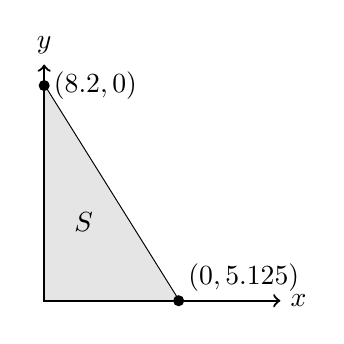
\begin{tikzpicture}
    \draw [thick] (1.708,0) coordinate (a_1) -- (0,2.733) coordinate (a_2);
    \path [fill=gray!20] (0,0) -- (a_2) to
        (a_1) -- (0,0);
    \draw [<->,thick] (0,3) node (yaxis) [above] {$y$} |- (3,0) node (xaxis) [right] {$x$};
    \fill[black] (a_1) circle (2pt) node[above right] {$(0, 5.125)$};
    \fill[black] (a_2) circle (2pt) node[right] {$(8.2, 0)$};
    \node at (0.5,1) {$S$};
\end{tikzpicture}
\caption{Feasible region $S$ defined by restrictions given in Eq. \ref{eq22}}\label{fig21}
\end{figure}

We define $g_i$ for $i \in \{1,2,3\}$ as follows.

\begin{equation}
\begin{aligned}
g_1(\mathbf{x}) &= 5x_1 + 8x_2 - 41\\
g_2(\mathbf{x}) &= x_1\\
g_3(\mathbf{x}) &= x_2\\
\end{aligned}
\label{eq23}
\end{equation}

Using Eq. \ref{eq21} and \ref{eq23}, $(\nabla f)_x$ and $(\nabla g_i)$ can be obtained as follows.

\begin{equation}
\begin{aligned}
(\nabla f)'_\mathbf{x} &= \begin{pmatrix} 2x_1 & 8x_2\end{pmatrix} \\
(\nabla g_1)'_\mathbf{x} &= \begin{pmatrix} 5 & 8\end{pmatrix} \\
(\nabla g_2)'_\mathbf{x} &= \begin{pmatrix} 1 & 0\end{pmatrix} \\
(\nabla g_3)'_\mathbf{x} &= \begin{pmatrix} 0 & 1\end{pmatrix} \\
\end{aligned}
\label{eq24}
\end{equation}

We claim $\mathbf{x} = (0,0)$ is an optimal point for function $f$. To prove this claim, we first need to show Fritz John necessary condition is satisfied; i.e. $F(f,\mathbf{x})$ and $FD(S,\mathbf{x_0})$ are disjoint.

For $\mathbf{x} = (0,0)$, constraints $g_2$ and $g_3$ are binding. We have $\mathbf{d} \in F(f,\mathbf{x}) \cap G(\mathbf{g}, \mathbf{x})$ if following conditions are satisfied, simultaneously.

\begin{equation}
\begin{aligned}
2x_1 d_1 + 8x_2 d_2 &< 0\\
x_1 d_1 &< 0\\
x_2 d_2 &< 0\\
\end{aligned}
\label{eq25}
\end{equation}

However, since $x_1 = x_2 = 0$, none of the conditions in Eq. \ref{eq25} are satisfied and therefore, $F(f,\mathbf{x}) \cap G(\mathbf{g}, \mathbf{x}) = \emptyset$ for $x = (0,0)$. Therefore we can continue with finding scalars $u_0$ and $u_i$ such that $u_0(\nabla f)_\mathbf{x} + \Sigma_{i=1}^{3} u_i (\nabla g_i)_\mathbf{x} = \mathbf{0}$. Using Eq. \ref{eq24}, this condition can be rewritten as follows.

\begin{equation}
u_0 \begin{pmatrix} 2x_1\\ 8x_2\\ \end{pmatrix} + u_2 \begin{pmatrix} 1\\ 0\end{pmatrix} + u_3 \begin{pmatrix} 0\\ 1\end{pmatrix} = \begin{pmatrix}
0 \\ 0 \end{pmatrix}
\label{eq26}
\end{equation}

For Eq. \ref{eq26} to hold for $x = (0, 0)$, we should have $u_i = 0$ for all $i\in \{1,2,3\}$ and $u_0$ can be chosen as any positive number. Since there is at least one positive scalar, all necessary conditions are satisfied for $\mathbf{x} = (0, 0)$ and $\mathbf{x}$ is proven to be the point of minimum for $f$.

\subsection*{Side Note}

In case the restrictions given in \ref{eq22} are changed to the following, the point of minimum of $f$ would be $\mathbf{x} = (5,2)$.

\begin{equation}
\begin{aligned}
5x_1 + 8x_2 - 41 &\geqslant 0,\\
x_1 &\geqslant 0,\\
x_2 &\geqslant 0.\\
\end{aligned}
\label{eq27}
\end{equation}

Choosing $\mathbf{x} = (5,2)$ will change the set of binding constraints to $\{g_1\}$. Therefore, \ref{eq25} will change to Eq. \ref{eq28}. In this case, $F(f,\mathbf{x}) \cap G(\mathbf{g}, \mathbf{x}) = \emptyset$ again, since no $d_1$ and $d_2$ exist to satisfy the following conditions simultaneously.

\begin{equation}
\begin{aligned}
10d_1 + 16d_2 &< 0,\\
5d_1 + 8d_2 &> 0\\
\end{aligned}
\label{eq28}
\end{equation}

Therefore, by showing there are $u_0$ and $u_i$ such that $u_0(\nabla f)_\mathbf{x} + \Sigma_{i=1}^{3} u_i (\nabla g_i)_\mathbf{x} = \mathbf{0}$, we can prove $\mathbf{x}(5,2)$ is really an optimal point. The former is easy to show, using Eq. \ref{eq29}.

\begin{equation}
u_0 \begin{pmatrix} 2x_1\\ 8x_2\\ \end{pmatrix} + u_1 \begin{pmatrix} 5\\ 8\end{pmatrix} = \begin{pmatrix}
0 \\ 0 \end{pmatrix}
\label{eq29}
\end{equation}

And replacing $x_1 = 5$, $x_2 = 2$, Eq. \ref{eq29} holds by having $u_0 = u_1 = 0$ and choosing $u_2$ and $u_3$ as any arbitrary positive number.
